\chapter{Specifikacija programske potpore}
		
	\section{Funkcionalni zahtjevi}
		
			\noindent \textbf{Dionici:}
			
			\begin{packed_enum}
				
				\item Neregistrirani korisnici
				\item Zaposlenici
				\item Revizori	
				\item Računovođe
				\item Direktor
				\item Razvojni tim
				
			\end{packed_enum}
			
			\noindent \textbf{Aktori i njihovi funkcionalni zahtjevi:}
			
			
			\begin{packed_enum}
				
				\item  \underbar{Neregistrirani korisnik (inicijator/sudionik) može:}
				\begin{packed_enum}
					
					\item Registrirati se u sustav
					
				\end{packed_enum}
			
				\item  \underbar{Zaposlenik (inicijator/sudionik) može:}
				
				\begin{packed_enum}
					
					\item Prijaviti se u sustav
					\item Učitati fotografiju u sustav te izvršiti konverziju te slike u dokument
					\item Učitati više fotografija od jednom u sustav te izvršiti njihovu konverziju u dokumente od jednom	
					\item Potvrditi ili odbiti točnost konverzije dokumenata u sustav
					\item Poslati dokument revizoru na pregled
					\item Pregledavati povijest svih dokumenata koje je zaposlenik unio u sustav
					
				\end{packed_enum}
			
				\item  \underbar{Revizor (inicijator/sudionik) može:}
				
				\begin{packed_enum}

					\item Provjeriti valjanost dokumenta kojeg mu je poslao zaposlenik
					\item Učitati fotografiju u sustav te izvršiti konverziju te slike u dokument 
					\item Učitati više fotografija od jednom u sustav te izvršiti njihovu konverziju u dokumente od jednom
					\item Potvrditi ili odbiti točnost konverzije dokumenata učitanih u sustav
					\item Potvrditi ili ispraviti automatsku kategorizaciju dokumenta
					\item Proslijediti dokument računovođi odgovornom za vrstu dokumenta kojoj dokument pripada
					\item Pregledati povijest svih dokumenata koje je revizor provjerio ili unio u sustav
					
				\end{packed_enum}
			
				\item  \underbar{Računovođa (inicijator/sudionik) može:}
				
				\begin{packed_enum}
					\item Računovođa može učitati jednu ili više slika u sustav te izvršiti njihovu konverziju u dokumente
					\item Potvrditi ili ispraviti automatsku kategorizaciju dokumenta
					\item Poslati dokumente direktoru na potpisivanje
					\item Arhivirati dokumente
					\item Pregledati povijest svih dokumenata one vrste za koju je računovođa zadužen
				\end{packed_enum}
			
				\item  \underbar{Direktor (inicijator/sudionik) može:}
			
				\begin{packed_enum}
					
					\item Potpisati dokument kojeg mu je poslao računovođa na potpisivanje
					\item Učitati jednu ili više fotografija u sustav te izvršiti njihovu konverziju u dokumente
					\item Potvrditi ili odbiti točnost konverzije dokumenata unesenih u sustav
					\item Potvrditi ili ispraviti automatsku kategorizaciju dokumenta
					\item Proslijediti dokument računovođi odgovornom za vrstu dokumenta kojoj dokument pripada
					
				\end{packed_enum}
			
			\end{packed_enum}
			
			\eject 
			
			
				
			\subsection{Obrasci uporabe}
					
				\subsubsection{Opis obrazaca uporabe}
					
	
					\noindent \underbar{\textbf{UC1 -Registracija}}
					\begin{packed_item}
	
						\item \textbf{Glavni sudionik:} Neregistrirani korisnik
						\item  \textbf{Cilj:} Registracija korisnika u sustav
						\item  \textbf{Sudionici:} Baza podataka
						\item  \textbf{Preduvjet:} -
						\item  \textbf{Opis osnovnog tijeka:}
						\item[] \begin{packed_enum}
	
							\item Neregistrirani korisnik odabire opciju za registraciju
							\item Neregistrirani korisnik unosi podatke za registraciju
							\item Korisnik prima obavijest o uspješnoj registraciji
							
						\end{packed_enum}
						
						\item  \textbf{Opis mogućih odstupanja:}
						\item[] \begin{packed_item}
	
							\item[2.a] Korisnik je odabrao već zauzetu ili neispravnu e-mail adresu, ili je dao ne dovoljno sigurnu lozinku
							\item[] \begin{packed_enum}
								
								\item Neregistriranog korisnika se vraća na stranicu za registraciju te ga se obavještava o neuspješnoj registraciji
								\item Korisnik mijenja nepravilne podatke ili odustaje od registracije	
							\end{packed_enum}
						\end{packed_item}
					\end{packed_item}
					
					
					\noindent \underbar{\textbf{UC2 - Prijava u sustav}}
					\begin{packed_item}
						
						\item \textbf{Glavni sudionik: } Korisnik sustava
						\item  \textbf{Cilj:} Prijava u sustav te pristup korisničkom sučelju
						\item  \textbf{Sudionici:} Baza podataka
						\item  \textbf{Preduvjet:}Registracija
						\item  \textbf{Opis osnovnog tijeka:}
						
						\item[] \begin{packed_enum}
							
							\item Korisnik odabire opciju za prijavu
							\item Korisnik unosi potrebne korisničke podatke
							\item Korisnik dobiva pristup korisničkom sučelju
						\end{packed_enum}
						
						\item  \textbf{Opis mogućih odstupanja:}
						
						\item[] \begin{packed_item}
							
							\item[2.a] Korisnik je upisao nepostojeće ili pogrešne korisničke podatke
							\item[] \begin{packed_enum}
								\item Korisnika se vraća na stranicu za prijavu te ga se obavještava o neuspjeloj prijavi
							\end{packed_enum}	
						\end{packed_item}
					\end{packed_item}
				
				\noindent \underbar{\textbf{UC3 -Promjena lozinke}}
				\begin{packed_item}
					
					\item \textbf{Glavni sudionik: } Korisnik
					\item  \textbf{Cilj:} Promjena lozinke koja se koristi pri prijavi u sustav
					\item  \textbf{Sudionici:} Baza podataka
					\item  \textbf{Preduvjet:} Registracija
					\item  \textbf{Opis osnovnog tijeka:}
					
					\item[] \begin{packed_enum}
						
						\item Korisnik bira opciju za promjenu lozinke
						\item Unosi staru lozinku kao potvrdu svog identiteta
						\item Bira novu lozinku te je upisuje dva puta
						\item Korisnik je obaviješten o uspješnoj promjeni lozinke
					\end{packed_enum}
					
					\item  \textbf{Opis mogućih odstupanja:}
					
					\item[] \begin{packed_item}
						
						\item[2.a] Korisnik je unio pogrešnu staru lozinku
						\item[] \begin{packed_enum}
							
							\item Korisnika se obavještava o pogrešnom unosu lozinke te ga se vraća na stranicu za promjenu lozinke
							\item Korisnik ponovno unosi staru lozinku ili odustaje od promjene lozinke
							
						\end{packed_enum}
					\end{packed_item}
				\end{packed_item}
				
				
				\noindent \underbar{\textbf{UC4 - Skeniranje jedne fotografije}}
				\begin{packed_item}
					
					\item \textbf{Glavni sudionik: }Korisnik
					\item  \textbf{Cilj:} Unijeti fotografiju u sustav te izvršiti njenu konverziju u dokument
					\item  \textbf{Sudionici:} Baza podataka
					\item  \textbf{Preduvjet:} Prijava u sustav
					\item  \textbf{Opis osnovnog tijeka:}
					
					\item[] \begin{packed_enum}
						
						\item Korisnik odabire opciju za učitavanje jedne fotografije
						\item Korisnik odabire fotografiju iz datotečnog sustava svog računala
						\item Korisnik dobiva obavijest o provedenoj konverziji
						
					\end{packed_enum}
					
					\item  \textbf{Opis mogućih odstupanja:}
					
					\item[] \begin{packed_item}
						
						\item[2.a] Korisnik je odabrao datoteku koja ne postoji na njegovom računalu
						\item[] \begin{packed_enum}
							
							\item Sustav obavještava korisnika o nastaloj pogrešci te ga preusmjerava na korisničko sučelje
							
						\end{packed_enum}
					\end{packed_item}
				\end{packed_item}
				
				\noindent \underbar{\textbf{UC5 -Skeniranje više fotografija}}
				\begin{packed_item}
					
					\item \textbf{Glavni sudionik: }Korisnik
					\item  \textbf{Cilj:} Unijeti više fotografija u sustav te izvršiti njihovu konverziju u dokumente
					\item  \textbf{Sudionici:} Baza podataka
					\item  \textbf{Preduvjet:} Prijava u sustav
					\item  \textbf{Opis osnovnog tijeka:}
					
					\item[] \begin{packed_enum}
						
						\item Korisnik odabire opciju za učitavanje više dokumenata
						\item Korisnik odabire više datoteka iz svog datotečnog sustava
						\item Korisnik dobiva obavijest o provedenim konverzijama
					
					\end{packed_enum}
					
					\item  \textbf{Opis mogućih odstupanja:}
					
					\item[] \begin{packed_item}
						
						\item[2.a] Jedna od fotografija koje je korisnik unio ne postoji u datotečnom sustavu
						\item[] \begin{packed_enum}
							
							\item Sustav provodi konverziju pronađenih dokumenata
							\item Sustav šalje korisniku obavijest o ne pronađenim dokumentima
							
						\end{packed_enum}
					\end{packed_item}
				\end{packed_item}
			
			
				\noindent \underbar{\textbf{UC6 -Potvrda ispravnosti konverzije}}
				\begin{packed_item}
					
					\item \textbf{Glavni sudionik: } Korisnik
					\item  \textbf{Cilj:} Potvrditi točnost konverzije dokumenta unesenih u sustav
					\item  \textbf{Sudionici:} Baza podataka
					\item  \textbf{Preduvjet:} Korisnik je prijavljen te je učitao jednu ili više fotografija u sustav
					\item  \textbf{Opis osnovnog tijeka:}
					
					\item[] \begin{packed_enum}
						
						\item Korisnik odabire opciju za potvrdu ispravnosti konverzije
						\item Korisniku se prikazuju fotografija i dokument generiran iz slike paralelno na ekranu, te mu se nudi opcija za prihvaćanje ili odbijanje točnosti konverzije
						 
						
					\end{packed_enum}
				\end{packed_item}
			
				\noindent \underbar{\textbf{UC7 -Prosljeđivanje dokumenata}}
				\begin{packed_item}
					
					\item \textbf{Glavni sudionik: }Korisnik
					\item \textbf{Cilj:} Proslijediti dokument potvrđene točnosti drugom korisniku s prikladnom razinom ovlasti za daljnju obradu dokumenta
					\item \textbf{Sudionici:} Baza podataka i drugi korisnici s višom razinom ovlasti
					\item \textbf{Preduvjet:} Korisnik je unio u sustav fotografiju, izvršio konverziju i potvrdio njenu točnost
					\item \textbf{Opis osnovnog tijeka:}
					
					\item[] \begin{packed_enum}
						
						\item Korisnik odabire opciju za slanje dokumenta
						\item Sustav prosljeđuje dokument odgovarajućem korisniku
						\item Korisnik dobiva obavijest o proslijeđenosti dokumenta
					\end{packed_enum}
				\end{packed_item}
			
				\noindent \underbar{\textbf{UC8 -Pregled vlastite povijesti}}
				\begin{packed_item}
					
					\item \textbf{Glavni sudionik: }Zaposlenik
					\item  \textbf{Cilj:} Pregled svih dokumenata koje je zaposlenik unio u sustav
					\item  \textbf{Sudionici:} Baza podataka
					\item  \textbf{Preduvjet:} Prijava
					\item  \textbf{Opis osnovnog tijeka:}
					
					\item[] \begin{packed_enum}
						
						\item Zaposlenik odabire opciju za pregled povijesti
						\item Aplikacija prikazuje korisniku listu svih dokumenata koje je unio u sustav
						\item Zaposlenik odabire dokument iz liste
						\item Aplikacija korisniku prikazuje dokument i sliku iz koje je dokument generiran
						
					\end{packed_enum}
				\end{packed_item}
			
			
		
			\noindent \underbar{\textbf{UC9 -Verifikacija točnosti konverzije}}
			\begin{packed_item}
				
				\item \textbf{Glavni sudionik: } Korisnik
				\item  \textbf{Cilj:} Potvrditi točnost generiranog dokumenta temeljem slike iz koje je dokument generiran
				\item  \textbf{Sudionici:} Baza podataka
				\item  \textbf{Preduvjet:} Skeniranje jedne ili više fotografija
				\item  \textbf{Opis osnovnog tijeka:}
				
				\item[] \begin{packed_enum}
					
					\item Korisnik odabire opciju za potvrdu konverzije
					\item Aplikacija korisniku prikazuje listu dokumenata čiju je točnost konverzije potrebno potvrditi
					\item Korisnik odabire dokument s liste, te mu aplikacija prikazuje dokument i sliku iz koje je dokument generiran. Dodatno aplikacija nudi mogućnost potvrde ili odbijanja točnosti konverzije
					\item Odabir korisnika o točnosti (ili netočnosti) konverzije pohranjuje se u bazu podataka
					
				\end{packed_enum}
			\end{packed_item}
		
			\noindent \underbar{\textbf{UC10 -Automatska kategorizacija dokumenata}}
			\begin{packed_item}
				
				\item \textbf{Glavni sudionik: }Revizor ili Računovođa ili Direktor
				\item  \textbf{Cilj:} Automatsko prepoznavanje vrste dokumenta pri konverziji dokumenta iz slike
				\item  \textbf{Sudionici:} Baza podataka
				\item  \textbf{Preduvjet:} Skeniranje jedne ili više fotografija
				\item  \textbf{Opis osnovnog tijeka:}
				
				\item[] \begin{packed_enum}
					
					\item Revizor ili Računovođa ili Direktor unose jednu ili više fotografija u sustav
					\item Sustav nakon konverzije automatski određuje kategoriju dokumenta
					\item Pri verifikaciji točnosti konverzije korisnicima se omogućuje i verifikacija točnosti automatske kategorizacije
					\item Nakon što je točnost automatske kategorizacije dokumenta potvrđena, kategorija dokumenta pohranjuje se u bazu podataka
				\end{packed_enum}
			\end{packed_item}
			
			\noindent \underbar{\textbf{UC11 -Slanje dokumenata na potpis}}
			\begin{packed_item}
				
				\item \textbf{Glavni sudionik: } Računovođa
				\item  \textbf{Cilj:} Slanje dokumenta Direktoru na potpis
				\item  \textbf{Sudionici:} Baza podataka, Direktor
				\item  \textbf{Preduvjet:} Prisutnost jednog ili više dokumenata koje treba obraditi u sustavu
				\item  \textbf{Opis osnovnog tijeka:}
				
				\item[] \begin{packed_enum}
					
					\item Računovođa bira jedan dokument iz liste dokumenata koje treba obraditi 
					\item Računovođa odabire opciju za slanje dokumenta za potpis
					\item Dokument je privremeno uklonjen iz liste dokumenata koje treba obraditi dok direktor ne potpiše dokument
				\end{packed_enum}
			\end{packed_item}
		
			\noindent \underbar{\textbf{UC12 -Arhiviranje}}
			\begin{packed_item}
				
				\item \textbf{Glavni sudionik: }Računovođa
				\item  \textbf{Cilj:} Arhiviranje dokumenata
				\item  \textbf{Sudionici:} Baza podataka
				\item  \textbf{Preduvjet:} Prisutnost jednog ili više dokumenata koji su spremni za arhiviranje
				\item  \textbf{Opis osnovnog tijeka:}
				
				\item[] \begin{packed_enum}
					
					\item Računovođa bira jedan ili više dokumenata iz liste dokumenata koje treba obraditi 
					\item Aplikacija nudi mogućnost za arhiviranje jednog ili više dokumenata
					\item Odabirom opcije za arhiviranje svi odabrani dokumenti dobivaju jedinstven broj arhiva
					\item Baza podataka pohranjuje jedinstven broj arhiva za svaki arhiviran dokument
					
				\end{packed_enum}
			\end{packed_item}
			
		
		
			\noindent \underbar{\textbf{UC13 -Pregled svih dokumenata određene kategorije}}
			\begin{packed_item}
				
				\item \textbf{Glavni sudionik: }Računovođa
				\item  \textbf{Cilj:} Pregled svih dokumenata određene kategorije koje su svi korisnici unijeli u sustav
				\item  \textbf{Sudionici:} Baza podataka
				\item  \textbf{Preduvjet:} Prisutnost jednog ili više dokumenata pretraživane kategorije u sustavu
				\item  \textbf{Opis osnovnog tijeka:}
				
				\item[] \begin{packed_enum}
					
					\item Računovođa odabire opciju za pregled povijesti svih dokumenata određene kategorije
					\item Aplikacije prikazuje računovođi listu svih dokumenata određene kategorije u sustavu
					\item Računovođa odabire dokument iz liste
					\item Aplikacija prikazuje računovođi dokument i sliku iz koje je dokument generiran
				\end{packed_enum}
			\end{packed_item}
			
			\noindent \underbar{\textbf{UC14 -Potpisivanje dokumenta}}
			\begin{packed_item}
				
				\item \textbf{Glavni sudionik: }Direktor
				\item  \textbf{Cilj:} Potpisivanje određenog dokumenta
				\item  \textbf{Sudionici:} Baza podataka
				\item  \textbf{Preduvjet:} Prisutnost jednog ili više dokumenata u sustavu za koje je zatražen potpis
				\item  \textbf{Opis osnovnog tijeka:}
				
				\item[] \begin{packed_enum}
					
					\item Direktor odabire opciju za potpisivanje dokumenata
					\item Aplikacija direktoru prikazuje listu dokumenata za koje je zatražen potpis
					\item Odabirom dokumenta aplikacija nudi direktoru opciju za potpis
					\item Direktor potpisuje dokument ili odbija potpisati dokument
				\end{packed_enum}
			\end{packed_item}
			
			\noindent \underbar{\textbf{UC15 - Promjena kategorije dokumenta}}
			\begin{packed_item}
				
				\item \textbf{Glavni sudionik: } Računovođa, Direktor, Revizor
				\item  \textbf{Cilj:} Promjena kategorije dokumenta kojeg su u sustav unijeli računovođa ili direktor
				\item  \textbf{Sudionici:} Baza podataka
				\item  \textbf{Preduvjet:} Prisutnost jednog ili više dokumenata u sustavu čija je ispravnost konverzije ispravna no automatska kategorizacija nije
				\item  \textbf{Opis osnovnog tijeka:}
				
				\item[] \begin{packed_enum}
					
					\item Direktor, računovođa ili revizor odabiru opciju za potvrdu ispravnosti automatske kategorizacije dokumenta
					\item Aplikacija prikazuje fotografija i dokument generiran iz fotografije te mu se nudi opcija za potvrdu točnosti ili promjenu kategorije dokumenta
					\item Baza podataka pohranjuje odabir korisnika
				\end{packed_enum}
			\end{packed_item}
			
			\noindent \underbar{\textbf{UC16 -Objava dokumenata na društvenoj mreži}}
			\begin{packed_item}
				
				\item \textbf{Glavni sudionik: } Direktor
				\item  \textbf{Cilj:} Objava dokumenata na društvenoj mreži
				\item  \textbf{Sudionici:} Baza podataka
				\item  \textbf{Preduvjet:} Prisutnost dokumenata u sustavu
				\item  \textbf{Opis osnovnog tijeka:}
				
				\item[] \begin{packed_enum}
					
					\item Direktor odabire opciju za objavu dokumenta na društvenoj mreži
					\item Direktor odabire na kojoj od ponuđenih društvenih mreža želi objaviti dokument
					\item Direktor unosi potrebne podatke za objavu dokumenta koje traži specifična društvena mreža
					\item Dokument se objavljuje na društvenoj mreži
					
				\end{packed_enum}
			\end{packed_item}
		
			\noindent \underbar{\textbf{UC17 -Pregled povijesti svih dokumenata}}
			\begin{packed_item}
				
				\item \textbf{Glavni sudionik: }Direktor
				\item  \textbf{Cilj:} Pregled povijesti svih dokumenata
				\item  \textbf{Sudionici:} Baza podataka
				\item  \textbf{Preduvjet:} Prisutnost dokumenata u sustavu
				\item  \textbf{Opis osnovnog tijeka:}
				
				\item[] \begin{packed_enum}
					
					\item Direktor odabire opciju za pregled povijesti dokumenata
					\item Aplikacija direktoru prikazuje listu svih dokumenata ikad unesenih u sustav
					\item Odabirom dokumenta sa liste prikazuje se fotografija i dokument generiran iz fotografije
				
				\end{packed_enum}
			\end{packed_item}
		
			\noindent \underbar{\textbf{UC18 -Brisanje dokumenta iz Arhiva}}
			\begin{packed_item}
				
				\item \textbf{Glavni sudionik: }Direktor
				\item  \textbf{Cilj:} Brisanje dokumenta iz Arhiva
				\item  \textbf{Sudionici:} Baza podataka
				\item  \textbf{Preduvjet:} Prisutnost jednog ili više arhiviranih dokumenata u sustavu
				\item  \textbf{Opis osnovnog tijeka:}
				
				\item[] \begin{packed_enum}
					
					\item Direktor odabire opciju za brisanje dokumenta iz arhiva
					\item Aplikacija prikazuje listu svih arhiviranih dokumenata, te direktor odabire onog kojeg želi učitati
					\item Direktor unosi svoju lozinku kao potvrdu svog identiteta i odluke
					\item Baza briše dokument iz sustava
					
				\end{packed_enum}
			\end{packed_item}
		
			\noindent \underbar{\textbf{UC19 -Pregled statistike zaposlenika}}
			\begin{packed_item}
				
				\item \textbf{Glavni sudionik: } Direktor 
				\item  \textbf{Cilj:} Pregled statistike zaposlenika
				\item  \textbf{Sudionici:} Baza podataka, korisnici
				\item  \textbf{Preduvjet:} Postojanje jednog ili više korisnika s razinom ovlasti manjom od direktor u sustavu
				\item  \textbf{Opis osnovnog tijeka:}
				
				\item[] \begin{packed_enum}
					
					\item Direktor odabire opciju za pregled statistike zaposlenika
					\item Aplikacija nudi listu svih korisnika
					\item Direktor odabire zaposlenika čije statistike želi pogledati
					\item Aplikacija prikazuje tražene podatke
				\end{packed_enum}
			\end{packed_item}
			
			\noindent \underbar{\textbf{UC20 -Promjena razine ovlasti}}
			\begin{packed_item}
				
				\item \textbf{Glavni sudionik: }Direktor 
				\item  \textbf{Cilj:} Promjena razine ovlasti korisnika
				\item  \textbf{Sudionici:} Baza podataka, korisnici
				\item  \textbf{Preduvjet:} Postojanje jednog ili više korisnika s razinom ovlasti manjom od direktor u sustavu
				\item  \textbf{Opis osnovnog tijeka:}
				
				\item[] \begin{packed_enum}
					
					\item Direktor odabire opciju za promjenu razine ovlasti korisnika
					\item Sustav prikazuje direktoru listu svih korisnika sustava
					\item Direktor odabire zaposlenika te mu dodjeljuje novu razinu ovlasti
					\item Baza podataka sprema unesene promjene
					
				\end{packed_enum}
			\end{packed_item}
			
			\noindent \underbar{\textbf{UC21 -Brisanje korisničkog računa}}
			\begin{packed_item}
				
				\item \textbf{Glavni sudionik: } Direktor
				\item  \textbf{Cilj:} Brisanje korisničkog računa
				\item  \textbf{Sudionici:} Baza podataka
				\item  \textbf{Preduvjet:} Registracija korisnika i prijava osobe s razinom ovalsti direktor u sustav
				\item  \textbf{Opis osnovnog tijeka:}
				
				\item[] \begin{packed_enum}
					
					\item Direktor bira opciju za brisanje korisničkog računa
					\item Direktoru se prikazuje lista svih korisnika sustava (osim njega samog) te odabire jednog korisnika s liste
					\item Direktor unosi svoju korisničku lozinku kao potvrdu svog odabira i identiteta
					\item Baza podataka briše korisnički račun
					\item Direktor dobiva obavijest o uspješnom brisanju korisničkog računa
				\end{packed_enum}
			\end{packed_item}
				
					
				\subsubsection{Dijagrami obrazaca uporabe}
					
					
				\begin{figure}[H]
					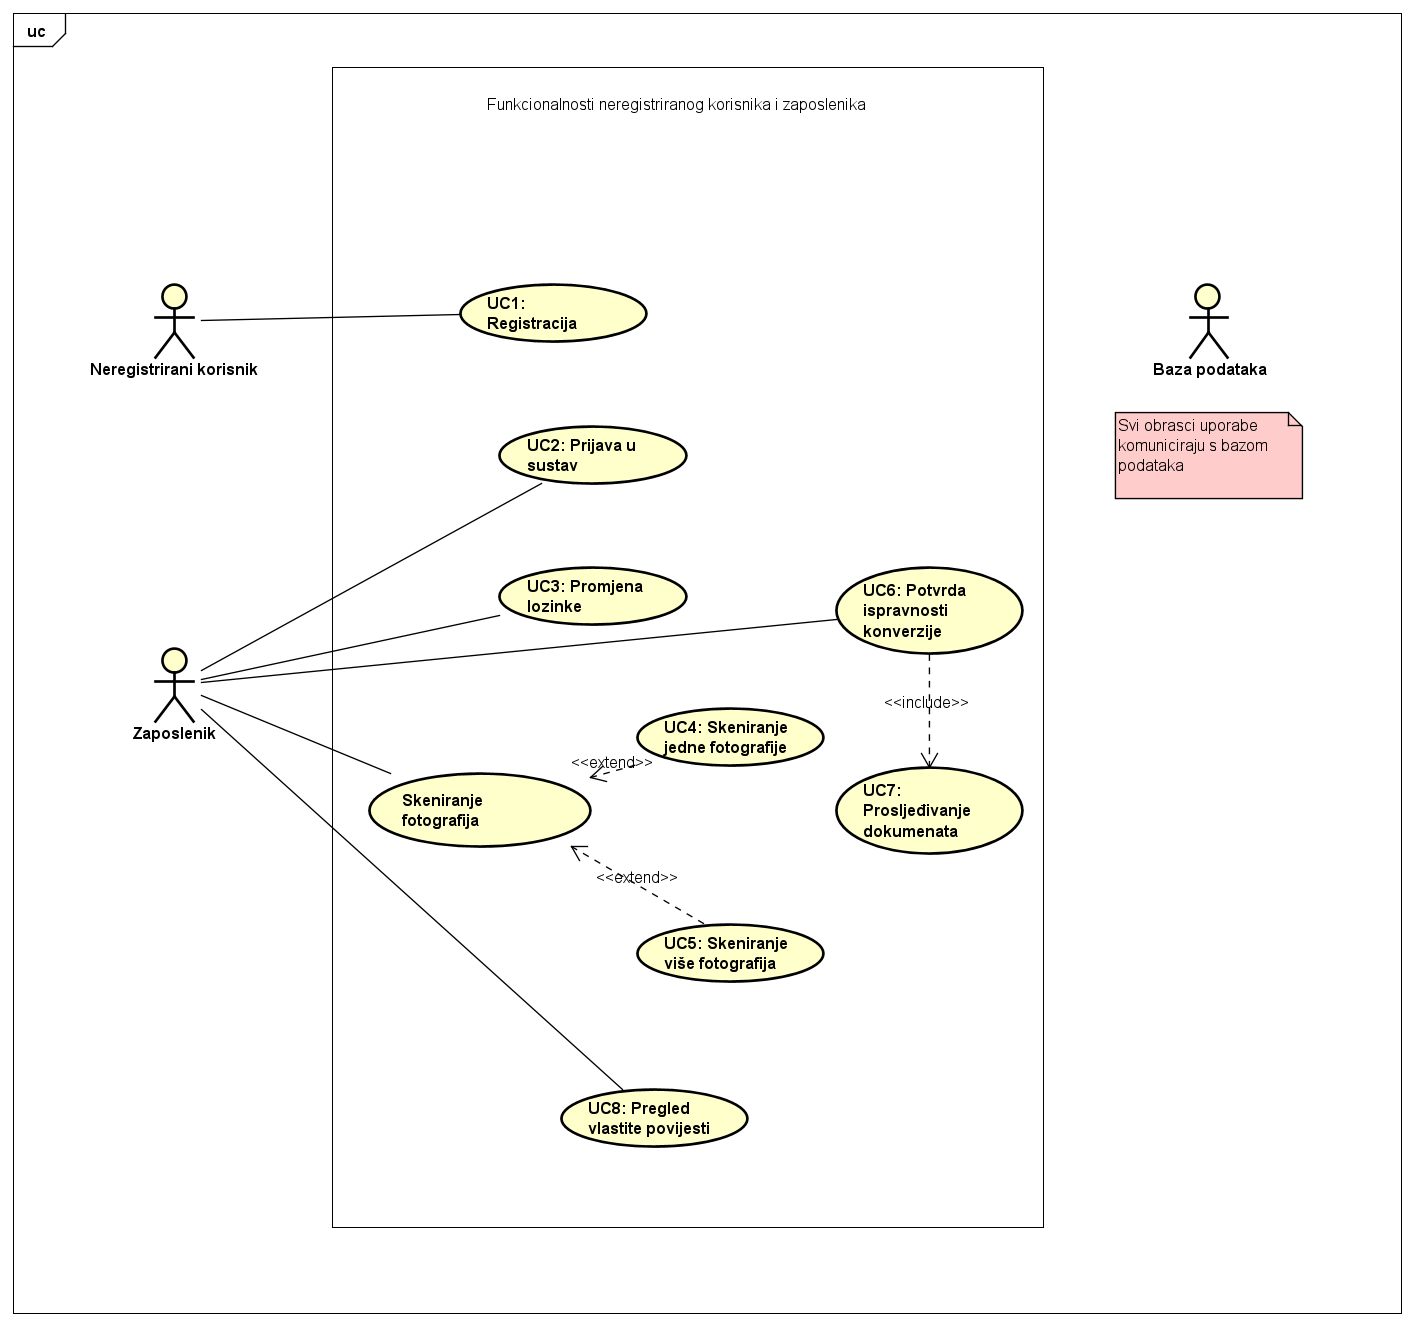
\includegraphics[scale=0.5]{slike/dijagram_obrasca_uporabe_1.PNG} %veličina slike u odnosu na originalnu datoteku i pozicija slike
					\centering
					\caption{Use case dijagram 1}
					\label{fig:promjene}
				\end{figure}
				
				\begin{figure}[H]
					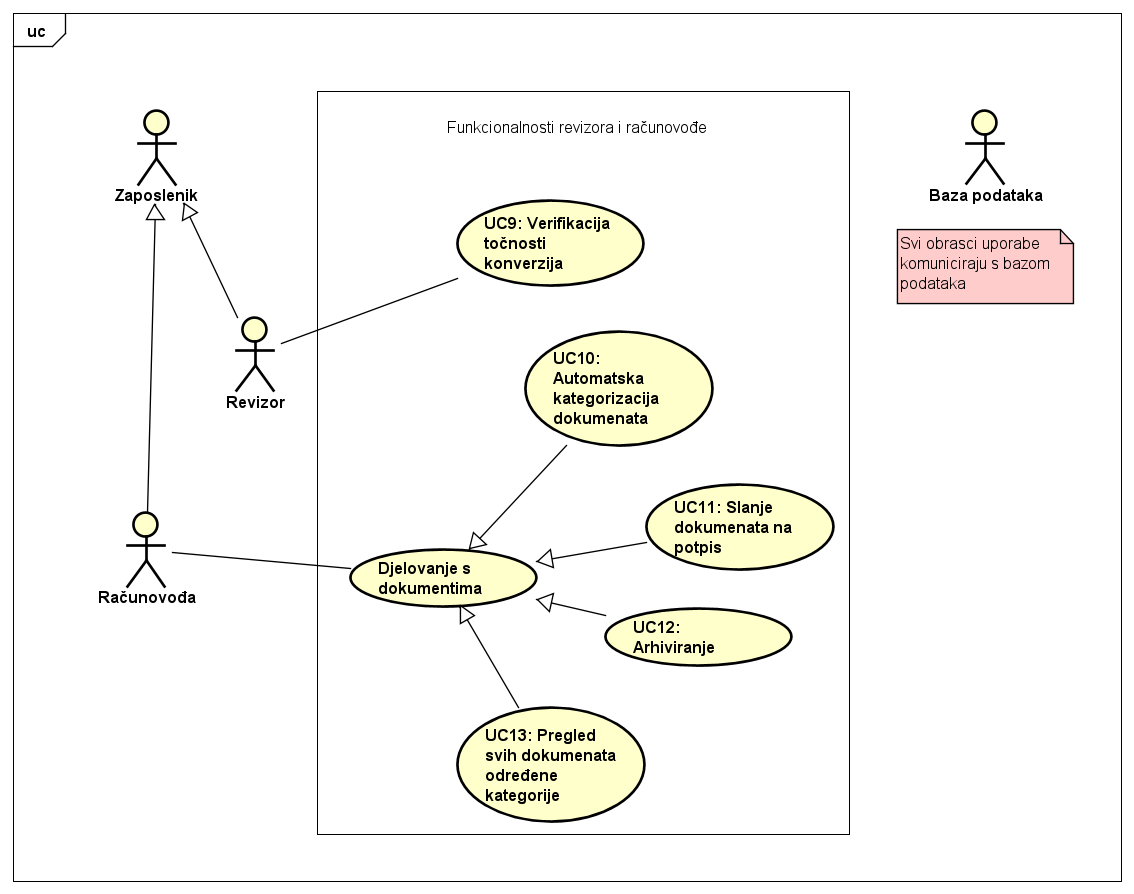
\includegraphics[scale=0.5]{slike/dijagram_obrasca_uporabe_2.PNG} %veličina slike u odnosu na originalnu datoteku i pozicija slike
					\centering
					\caption{Use case dijagram 2}
					\label{fig:promjene}
				\end{figure}		
				
				\begin{figure}[H]
					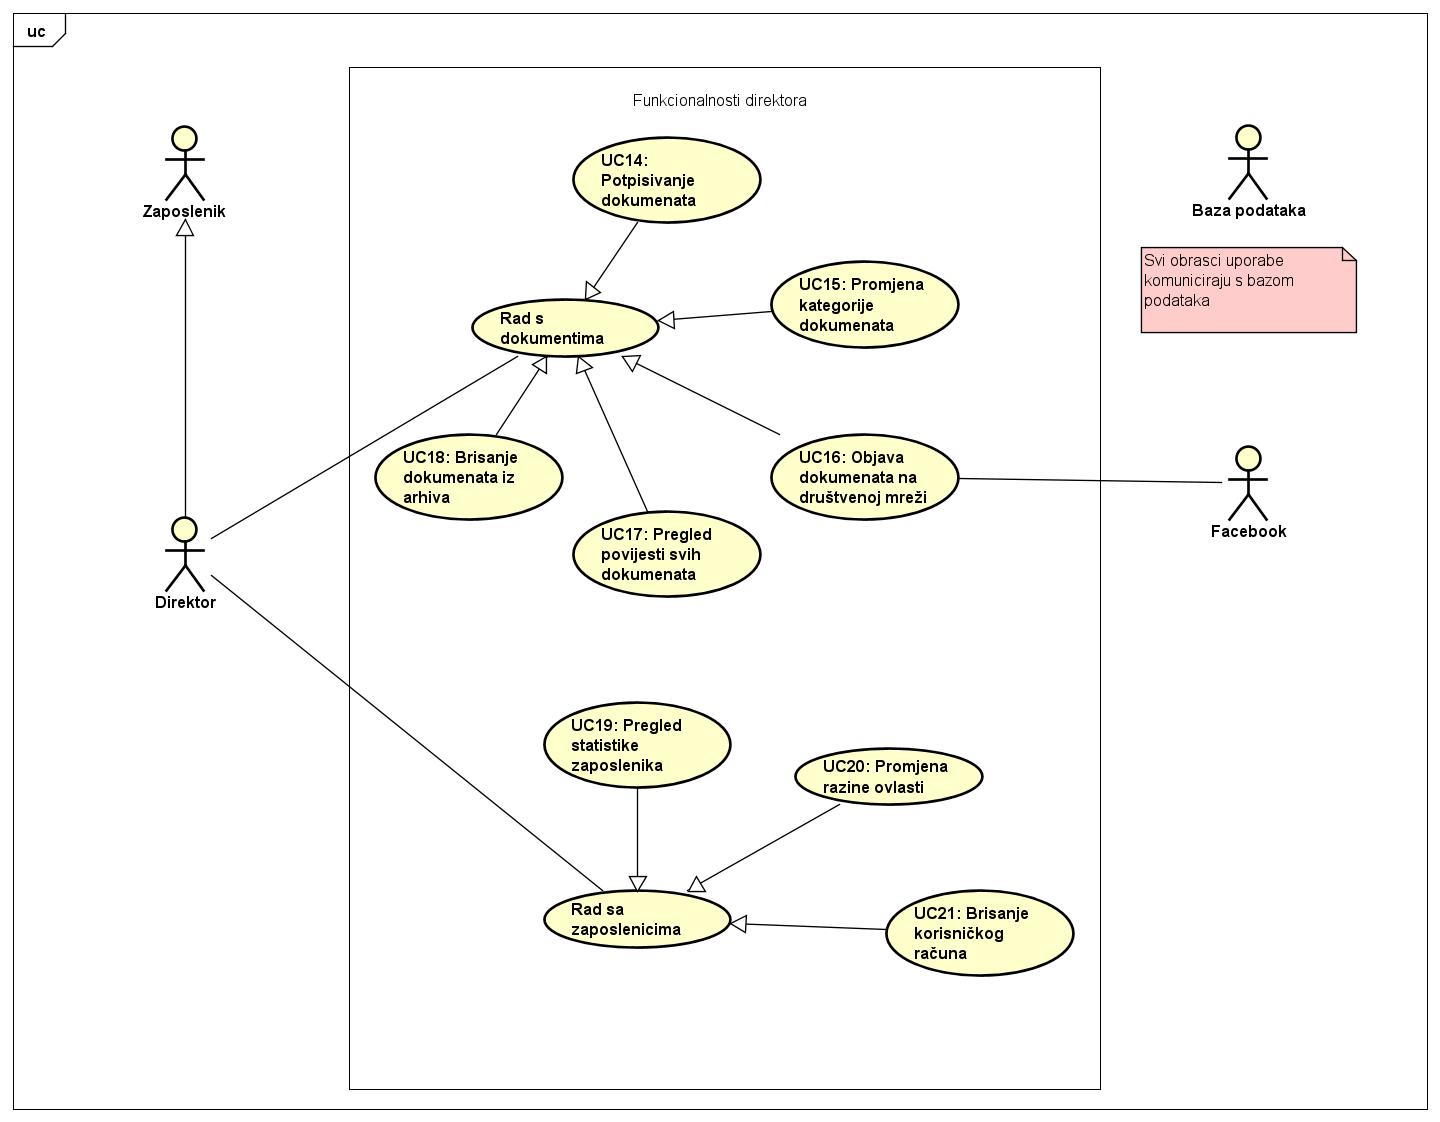
\includegraphics[scale=0.4]{slike/dijagram_obrasca_uporabe_3.PNG} %veličina slike u odnosu na originalnu datoteku i pozicija slike
					\centering
					\caption{Use case dijagram 3}
					\label{fig:promjene}
				\end{figure}
				
			\subsection{Sekvencijski dijagrami}
				
				\begin{figure}[H]
					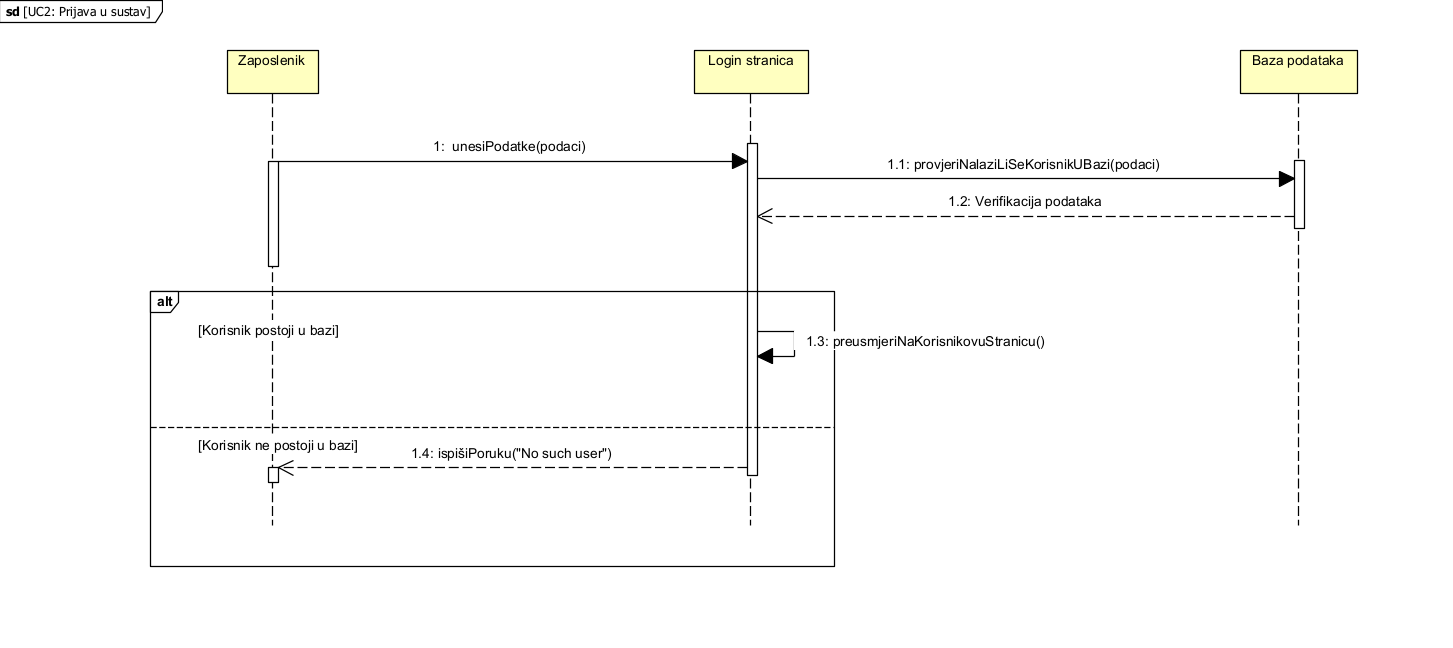
\includegraphics[scale=0.5]{slike/sd1.PNG} %veličina slike u odnosu na originalnu datoteku i pozicija slike
					\centering
					\caption{Sekvencijski dijagram 1 - Login}
					\label{fig:promjene}
				\end{figure}

				\begin{figure}[H]
					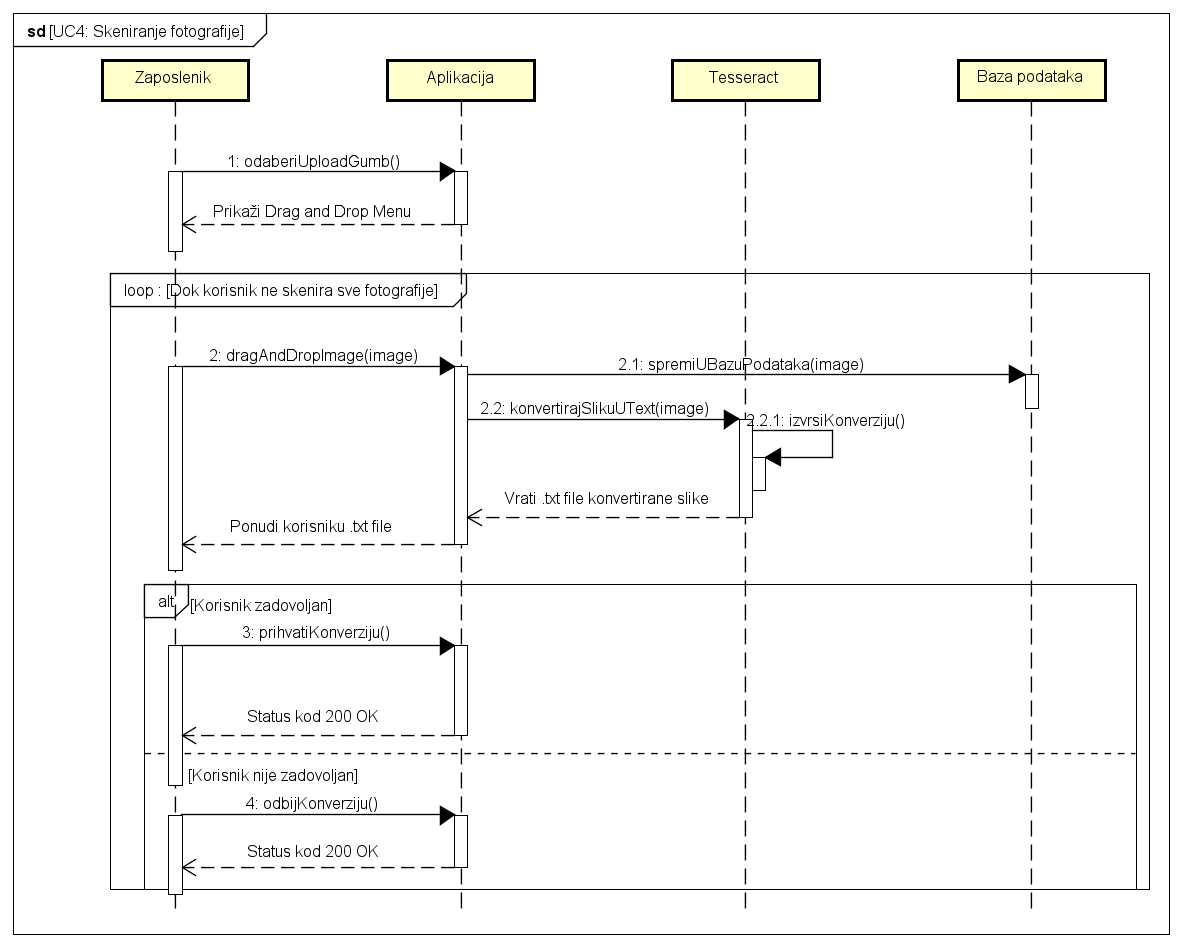
\includegraphics[scale=0.5]{slike/uc4_skeniranje_fotografije.PNG} %veličina slike u odnosu na originalnu datoteku i pozicija slike
					\centering
					\caption{Sekvencijski dijagram 2 - Skeniranje fotografija}
					\label{fig:promjene}
				\end{figure}

				\begin{figure}[H]
					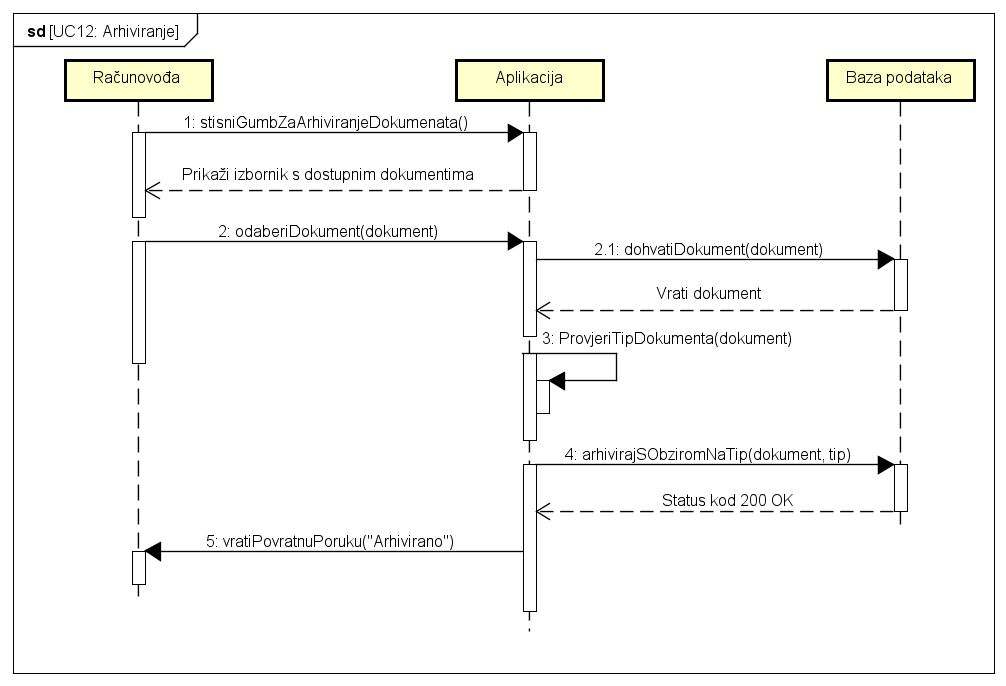
\includegraphics[scale=0.5]{slike/uc12_arhiviranje.PNG} %veličina slike u odnosu na originalnu datoteku i pozicija slike
					\centering
					\caption{Sekvencijski dijagram 3 - Arhiviranje}
					\label{fig:promjene}
				\end{figure}

				\begin{figure}[H]
					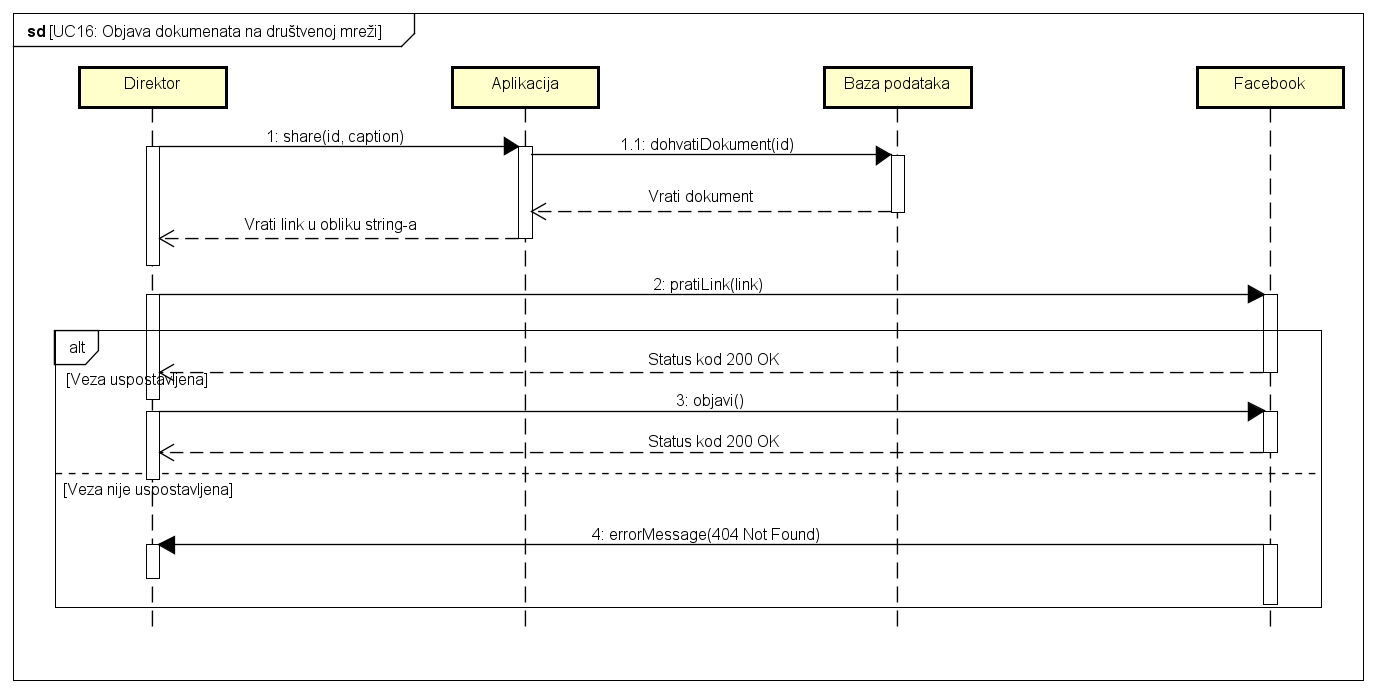
\includegraphics[scale=0.5]{slike/uc16_objava_dokumenata_na_drustvenoj_mrezi.PNG} %veličina slike u odnosu na originalnu datoteku i pozicija slike
					\centering
					\caption{Sekvencijski dijagram 4 - Objava dokumenata na društvenoj mreži}
					\label{fig:promjene}
				\end{figure}
	
		\section{Ostali zahtjevi}
		
		\begin{packed_item}
			\item Korisničko sučelje mora podržavati čitavu hrvatsku abecedu
			
			\item Odgovor na HTTP zahtjev ne smije trajati duže od nekoliko sekundi
			
			\item Aplikacija mora podržati rad više korisnika istovremeno
			
			\item Korisničko sučelje mora biti jasno i jednostavno za upotrebu
			
			\item Sustav mora biti implementiran kao web-aplikacija
			
			\item Sustavu se mora putem HTTPS protokola moći pristupiti s javne mreže
			
			\item Nadogradnja sustava ne smije narušiti postojeće funkcionalnosti
			
			\item Mora postojati mogućnost brze i učinkovite nadogradnje sustava
			
		\end{packed_item}
		
			
			 
			 
			 
	